\section{The soft curb}\label{sec:soft}

In this section ``free'', ``parked'' and ``lane configuration'' refer to the soft-curb model of \cref{sec:model-soft}.
The curb now constrains only the tyres.
Two tyre points matter: the outer rear corner of the curb-side rear tyre and the outer front corner of the curb-side front tyre,
\[
  \cTr=P-\lambda\,\e-T_o\,\n,\qquad \cTf=P+a\,\e-T_o\,\n,\qquad a:=d_w+\lambda .
\]
For $\psi\in[0,\pi/2]$ the lowest point of $\W(q)$ is $\cTr$, and for $\psi\in[-\pi/2,0]$ it is $\cTf$.
In analogy with $r$ and $\beta$ we put
\[
  r_t=\sqrt{\lambda^2+(R+T_o)^2},\qquad (\cos\beta_t,\sin\beta_t)=\frac{(R+T_o,\lambda)}{r_t},
\]
so that $\cTr=C+r_t\,\e(\psi-\tfrac\pi2-\beta_t)$ and $\cTr_y=C_y-r_t\cos(\psi-\beta_t)$.

\subsection{Parked cars}
If $H<\min(b+\lambda,\,d_b+a)$, let $\psi_t$ and $\psi_t'$ be the roots in $(0,\pi/2)$ of
\[
  (b+\lambda)\sin\psi+(w-\delta_s)\cos\psi=H\qquad\text{and}\qquad(d_b+a)\sin\psi+(w-\delta_s)\cos\psi=H ,
\]
respectively, and put $\psi_{\max}=\max(\psi_t,\psi_t')$.
The roots are unique, because each left side increases from $w-\delta_s<H$ and then decreases to $b+\lambda>H$, respectively $d_b+a>H$.

\begin{lemma}[parked cars, soft curb]\label{lem:soft-fit}
Assume $H<\min(b+\lambda,\,d_b+a)$.
If $q$ is parked, then modulo $2\pi$ either $\psi\in[-\psi_t',\psi_t]$ or $\psi\in[\pi-\psi_t,\pi+\psi_t']$.
Assume moreover
\begin{equation}\label{eq:soft-band}
  (w-\delta_s)\cos\psi_{\max}-\max(d_b,d_f)\sin\psi_{\max}>m ,
\end{equation}
and let $q$ be parked with $\psi\in[-\psi_t',\psi_t]$.
\begin{enumerate}[label=(\alph*)]
\item If $\psi\ge0$, then $C_x\ge X(\psi)$ and $r_t\cos(\psi-\beta_t)\le C_y\le H+Y(\psi)$.
\item If $\psi<0$, then $C_x\ge d_b\cos\psi+\Rm|\sin\psi|$, $C'_x\ge d_b\cos\psi-\Rp|\sin\psi|$ and $r_t\cos(\psi-\beta_t)\le C_y\le H+\Rm\cos\psi-d_b|\sin\psi|$.
\item $\cFL_x\le L$.
\end{enumerate}
\end{lemma}

\begin{proof}
For $\psi\in[0,\pi/2]$ the lowest point of $\W(q)$ is $\cTr$ and the highest point of $\fp(q)$ is $\cFL$.
Since $\cFL-\cTr=(b+\lambda)\e+(w-\delta_s)\n$, the conditions $\cTr_y\ge0$ and $\cFL_y\le H$ give $(b+\lambda)\sin\psi+(w-\delta_s)\cos\psi\le H$, hence $\psi\le\psi_t$.
For $\psi\in[-\pi/2,0]$ the same argument with $\cTf$ and $\cRL$, where $\cRL-\cTf=-(d_b+a)\e+(w-\delta_s)\n$, gives $|\psi|\le\psi_t'$.
For the other headings the two sides of the car exchange their roles: then the lowest tyre point is a corner of a lane-side tyre and the highest body point is a curb-side corner.
The same computation gives $\psi\in[\pi-\psi_t,\pi+\psi_t']$.

(a) We have $\cTr_y\ge0$ and $\cFL_y\le H$.
Moreover $\cRL_y=\cTr_y+(w-\delta_s)\cos\psi-(d_b-\lambda)\sin\psi>m$ by \eqref{eq:soft-band}.
So $\cRL$ lies in the band or on its upper boundary, and as in \cref{lem:parked} we get $\cRL_x\ge0$, i.e.\ $C_x\ge X(\psi)$.
The upper bound for $C_y$ comes from $\cFL_y\le H$ and the lower bound from $\cTr_y\ge0$.
(b) Now $\cRL$ is the highest point, and $\cRL_y=\cTf_y+(d_b+a)|\sin\psi|+(w-\delta_s)\cos\psi>m$.
So again $\cRL_x\ge0$, and the bounds follow as in \cref{lem:parked}(b) and (a).
(c) We have $\cFL_y\le H$.
For $\psi\ge0$, $\cFL_y=\cTr_y+(b+\lambda)\sin\psi+(w-\delta_s)\cos\psi>m$.
For $\psi<0$, the identity $\cFL-\cTf=(d_f-\lambda)\e+(w-\delta_s)\n$ and \eqref{eq:soft-band} give $\cFL_y>m$.
Hence $\cFL$ lies in the band or on its upper boundary, and $\cFL_x\le L$ by continuity.
\end{proof}

By \cref{lem:mirror} we may assume that an exit starts at a parked configuration with $\psi\in[-\psi_t',\psi_t]$.

\subsection{One manoeuvre}
The optimal exit has the shape of the one in \cref{thm:one}, but it starts from a more strongly tilted position.
The tilt is now limited by the rear tyre touching the curb at rest, rather than by the swing of the rear corner during the exit.
Define $\psi_b^{\rm s},\psi_n^{\rm s}\in(0,\pi/2)$ and $\eta$ by
\[
  \sin\psi_b^{\rm s}=\frac{H+\delta_s}{b+\lambda},\qquad \sin\psi_n^{\rm s}=\frac{H+\delta_s}{a},\qquad \eta=(d_f-\lambda)\sin\gamma+\delta_s ,
\]
and let $\psi_u^{\rm s}\in(0,\pi/2)$ solve $(R-T_o)(1-\cos\psi_u^{\rm s})+\lambda\sin\psi_u^{\rm s}=H+\delta_s$.
Put
\[
  h_0=H-(w-\delta_s)\cos\psi_{\max},\qquad h_1=\frac{Ha}{a+d_b},\qquad \Gamma(z)=\sqrt{a^2-z^2}-a\log\frac{a+\sqrt{a^2-z^2}}{z},
\]
and, with $f_b(\psi)=d_b\cos\psi-\tfrac w2\sin\psi$ as in \eqref{eq:Bback},
\begin{equation}\label{eq:Bback-soft}
  B^{\rm s}_{\rm back}=b\cos\psi_{\max}-\tfrac w2\sin\psi_{\max}+\min\big(f_b(-\psi_n^{\rm s}),f_b(\psi_u^{\rm s})\big)+\frac{R}{R+T_o}\big(\Gamma(h_1)-\Gamma(h_0)\big).
\end{equation}
Finally let
\[
  \varphi_0(\psi)=X(\psi)+\sqrt{\rho^2-Y(\psi)^2},
\]
which is the function $\varphi_{\rm c}$ of the proof of \cref{prop:one-forward} without its curb-cost term.

\begin{assumption}\label{ass:soft}
\leavevmode
\begin{enumerate}[label=(S\arabic*),nosep]
\item\label{S:db} $d_b<b$ and $\lambda\le\min(d_b,d_f)$;
\item\label{S:fit} $H+\delta_s<\min(b+\lambda,\,d_b+a,\,\lambda+R-T_o)$, $\psi_{\max}<\gamma$, \eqref{eq:soft-band}, $(w-\delta_s)\cos\psi_b^{\rm s}>m$, $\Rp\cos\psi_t>\Rm$, $\Rm\ge d_b\tan(\psi_t'/2)$, $\Rm\tan\psi_t'<b$, $r_t\cos(\psi_{\max}+\beta_t)\ge H$ and $h_0<h_1$;
\item\label{S:nose} $2Rb>w\rho$, $m\rho+(d_f-\lambda)\Rp<(w-\delta_s)b$ and $b\rho>(H+\eta)\Rp$;
\item\label{S:swing} $\lambda\le\big(H+Y(\psi_t)\big)\sin\psi_t$;
\item\label{S:min} $\cos\psi_t\sqrt{b^2+2Rw}>\Rm\sin\psi_t+b$;
\item\label{S:end} $Y(\psi_t)\ge d_b$;
\item\label{S:far} $d_b\cos\psi_{\max}-\Rp\sin\psi_{\max}+\rho\ge\Lambda_1^{\rm s}$ and $B^{\rm s}_{\rm back}\ge\Lambda_1^{\rm s}$, where $\Lambda_1^{\rm s}=\varphi_0(\psi_t)$ as in \eqref{eq:Lam1soft} below.
\end{enumerate}
\end{assumption}

These conditions are checked by the script \texttt{numerics/soft\_theory.py}.
They hold for the typical car, and for the compact car, the mid-size sedan, the large SUV and the van of \cref{tab:cars}.
For the city car only \ref{S:swing} fails, by a narrow margin (see below).

\begin{theorem}[one manoeuvre, soft curb]\label{thm:one-soft}
Under \cref{ass:soft},
\begin{equation}\label{eq:Lam1soft}
  \Lmins(1)=\Lambda_1^{\rm s}:=\varphi_0(\psi_t)=X(\psi_t)+\sqrt{\rho^2-Y(\psi_t)^2}.
\end{equation}
An optimal exit starts from the parked configuration $q_t$ with heading $\psi_t$, $\cFL_y=H$ and $\cRL_x=0$, whose rear tyre touches the curb ($\cTr_y=0$).
It drives forward with full left lock, during which its front curb-side corner grazes $\Qf$, and then straightens with full right lock.
\end{theorem}

In the same notation, \cref{thm:one} says $\Lmin(1)=\varphi_0(\psi_d)$.
The two optimal exits differ only in the tilt of the starting position.
Since $\varphi_0$ is decreasing on the relevant range, the larger tilt gives the shorter slot.
For the typical car $\psi_t=0.0561$ rad $=3.21^\circ$, against $\psi_d=1.80^\circ$, and $\Lambda_1^{\rm s}=5.809$ m, against $\Lambda_1=5.833$ m.
In the optimal position the rear curb-side corner overhangs the curb by $5.8$ cm.
Further $\psi_t'=0.0577$, $\beta_t=0.0545$, $\psi_b^{\rm s}=0.565$, $\psi_n^{\rm s}=0.782$, $\psi_u^{\rm s}=1.187$ and $B^{\rm s}_{\rm back}=7.34$ m.
For the city car, during the exit from $q_t$ the outer rear corner of the tyre would dip $0.025$ mm below the curb.
There the numerical optimum, $4.89485$ m, exceeds $\varphi_0(\psi_t)=4.89480$ m by less than $0.1$ mm.

\begin{proof}
We follow \cref{sec:one} and list the changes.
By \cref{lem:mirror,lem:soft-fit} we may assume that an exit starts with $\psi(0)\in[-\psi_t',\psi_t]$.

\emph{Upper bound.}
Let $L=\Lambda_1^{\rm s}$ and $q_t=(P,\psi_t)$ with $P=(d_b\cos\psi_t+\tfrac w2\sin\psi_t,\ H-b\sin\psi_t-\tfrac w2\cos\psi_t)$.
Then $\cFL_y=H$ and $\cRL_x=0$.
By the definition of $\psi_t$, $\cTr_y=\cFL_y-(b+\lambda)\sin\psi_t-(w-\delta_s)\cos\psi_t=0$.
The left centre is $C=(X(\psi_t),\,H+Y(\psi_t))$, and $\Qf$ lies on the circle of radius $\rho$ about $C$.
The proof of \cref{prop:one-upper} applies with the following changes.
\begin{itemize}[nosep]
\item The configuration $q_t$ is parked.
Its lowest tyre point $\cTr$ is on the curb, and the footprint lies in $\{y\le H\}\cap\{x\ge0\}$ with $\cFC_x<L$, exactly as there.
\item During the first arc no point of the footprint enters $\Or$.
All points start below $C$, because $C_y=H+Y(\psi_t)>H$ by \ref{S:end}.
A point below $C$ moves to the right and so keeps $x\ge0$; once it rises above $C$ it is in the lane.
(This argument also makes the condition $X(\psi_d)\ge0$ in \cref{prop:one-upper} unnecessary.)
\item For the tyres, a point with body coordinates $(u,v)$ descends during the arc only while $\tan\psi<-u/(R-v)$.
For $\psi\ge\psi_t$ this requires $u<0$ and $R-v<\lambda/\tan\psi_t$, so the point is at distance less than $\lambda/\sin\psi_t$ from $C$.
Its height therefore stays above $C_y-\lambda/\sin\psi_t\ge0$ by \ref{S:swing}; all other tyre points rise.
\item At heading $\pi/2$ a body point $(u,v)$ is at height $C_y+u\ge H+Y(\psi_t)-d_b\ge H$ by \ref{S:end}.
\end{itemize}
The second arc is as in \cref{prop:one-upper}.

\emph{Forward exits.}
Let a forward manoeuvre lead from a parked configuration $q_0$ with $\psi(0)\in[-\psi_t',\psi_t]$ to a lane configuration, and suppose $L<\Lambda_1^{\rm s}$.
Steps 1--7 of the proof of \cref{prop:one-forward} go through with the following changes.
The curb enters there only through lower bounds for the heights of points.
\begin{itemize}[nosep]
\item Step 2(i): from $\cTr_y\ge0$ and $\cFC-\cTr=(b+\lambda)\e-\delta_s\n$ we get $\cFC_y\ge(b+\lambda)\sin\psi-\delta_s$.
So for $s<\tau$ the heading satisfies $\psi<\psi_b^{\rm s}$ whenever $\psi\in[0,\pi/2]$; in (ii) and below, $\psi_b$ is replaced by $\psi_b^{\rm s}$.
In (iii), $\cRL_x(0)\ge0$ (\cref{lem:soft-fit}) gives $C'_x(0)=P_x(0)+R\sin\psi(0)\ge d_b\cos\psi(0)+\Rp\sin\psi(0)\ge d_b\cos\psi_{\max}-\Rp\sin\psi_{\max}$, and $\psi(0)>-\gamma$ by \ref{S:fit}.
\item The case $\psi(t)=-\gamma$: now $\cFL_x(t)\ge d_b\cos\psi_{\max}-\Rp\sin\psi_{\max}+\rho\ge\Lambda_1^{\rm s}>L$ by \ref{S:far}, and $\cFL_y(t)<H$ as before.
If $\cFL_y(t)\le m$, then, since $\cTf-\cFL=-(d_f-\lambda)\e-(w-\delta_s)\n$,
\[
  \cTf_y=\cFL_y+(d_f-\lambda)\sin\gamma-(w-\delta_s)\cos\gamma\le m+\frac{(d_f-\lambda)\Rp-(w-\delta_s)b}{\rho}<0
\]
by \ref{S:nose}, and the front tyre meets the curb.
\item Step 5 with $\psi\ge0$ needs $\cFL_y>m$.
This now follows from $\cFL_y=\cFC_y+w\cos\psi\ge(w-\delta_s)\cos\psi>m$ for $\psi\in[0,\psi_b^{\rm s}]$, by \ref{S:fit}.
\item Step 5 with $\psi<0$: the case $\cFL_y\le m$ is excluded as in the previous item, because $(d_f-\lambda)|\sin\psi|-(w-\delta_s)\cos\psi$ increases with $|\psi|<\gamma$.
Since $\cFC-\cTf=(d_f-\lambda)\e-\delta_s\n$, we have $\cFC_y\ge-\eta$.
So the bound $(H-\cFC_y)|\sin\psi|\le H\sin\gamma$ becomes $(H-\cFC_y)|\sin\psi|\le(H+\eta)\sin\gamma<b$, by \ref{S:nose}.
\item Of Step 7 only the first statement is needed: $|C-\Qf|$ is non-increasing on $[0,\tau]$.
\end{itemize}
Steps 8 and 9 are replaced by a simpler argument, which needs no curb cost.
By Steps 6 and 7, $|C(0)-\Qf|\ge|C(\tau)-\Qf|\ge\rho$.
By \cref{lem:soft-fit} and \ref{S:fit}, $C_y(0)\ge r_t\cos(\psi_{\max}+\beta_t)\ge H$.
Also $C_x(0)=\cFL_x-b\cos\psi(0)-\Rm\sin\psi(0)<L$, because $\Rm\tan\psi_t'<b$.
Hence
\[
  L\ \ge\ C_x(0)+\sqrt{\rho^2-(C_y(0)-H)^2},
\]
and the right side increases with $C_x(0)$ and decreases with $C_y(0)\ge H$.
If $\psi(0)\in[0,\psi_t]$, \cref{lem:soft-fit}(a) gives $L\ge\varphi_0(\psi(0))$.
If $\psi(0)<0$, \cref{lem:soft-fit}(b) gives $C_x(0)\ge d_b\cos\psi+\Rm|\sin\psi|\ge d_b$, because $\Rm\ge d_b\tan(\psi_t'/2)$, and $C_y(0)\le H+\Rm$; so $L\ge\varphi_0(0)$.
Finally, $\varphi_0$ is decreasing on $[0,\psi_t]$.
There $d_b\le Y\le\Rm$ by \ref{S:end}, and as in Step 9 the derivative is at most $-\Rm\cos\psi_t+\Rm(\Rm\sin\psi_t+b)/\sqrt{b^2+2Rw}<0$, by \ref{S:min}.
Hence $L\ge\varphi_0(\psi_t)=\Lambda_1^{\rm s}$, a contradiction.

\emph{Reverse exits.}
Let a reverse manoeuvre lead from a parked configuration with $\psi(0)\in[-\psi_t',\psi_t]$ to a lane configuration.
We show $L\ge B^{\rm s}_{\rm back}$, following \cref{prop:one-reverse} with
\[
  h=P_y-T_o\cos\psi ,
\]
the height of the outer sidewall of the curb-side rear tyre at the axle.
Now $h'=-\sin\psi\,(1-T_o\psi')$ with $1-T_o\psi'\in[1-T_o/R,\,1+T_o/R]$, so $h$ increases only while $\psi<0$.
Let $\tau_r$ be the first time with $\cRC_y=H$.
\begin{itemize}[nosep]
\item The highest point of the parked car, $\cFL$ or $\cRL$, is at height at most $H$.
Hence $h(0)\le H-(w-\delta_s)\cos\psi(0)\le h_0$.
\item On $[0,\tau_r)$ we have $h<H+\delta_s$.
While $\psi<0$ this follows from $\cRC_y=h+d_b|\sin\psi|-\delta_s\cos\psi<H$, and while $\psi\ge0$ the height $h$ does not increase.
\item If $\psi\le0$, then $\cTf_y=h-a|\sin\psi|\ge0$, so $|\sin\psi|\le h/a<\sin\psi_n^{\rm s}$.
\item The function $C'_y=h-(R-T_o)\cos\psi$ does not increase while $\psi\ge0$.
Suppose $\psi$ first reached $\psi_u^{\rm s}$ at a time $t$.
The argument of \cref{prop:one-reverse} would give $h(t)<H+\delta_s-(R-T_o)(1-\cos\psi_u^{\rm s})=\lambda\sin\psi_u^{\rm s}$; if the positive excursion starts at time $0$, it uses $\Rp\cos\psi_t>\Rm$.
This contradicts $\cTr_y=h(t)-\lambda\sin\psi_u^{\rm s}\ge0$.
\end{itemize}
Hence $\psi\in(-\psi_n^{\rm s},\psi_u^{\rm s})$ on $[0,\tau_r]$.
At $\tau_r$ we have $h(\tau_r)\ge h_1$.
Indeed, if $\psi\le0$ then $H=\cRC_y\le h+d_b|\sin\psi|\le h(1+d_b/a)$, and if $\psi>0$ then $H<h$.

The Gronwall step is replaced by a sharper estimate.
Let $g(z)=\sqrt{a^2-z^2}/z$, so that $\Gamma'=g$ on $(0,a]$.
Let $s_0$ be the last time in $[0,\tau_r]$ with $h\le h_0$; on $[s_0,\tau_r]$ we have $h_0\le h<H+\delta_s<a$.
While $\psi<0$, the bounds $h'\le(1+T_o/R)|\sin\psi|$ and $|\sin\psi|\le h/a$ give
\[
  \frac{\dd}{\dd s}\Gamma(h)=g(h)\,h'\ \le\ \frac{R+T_o}{R}\sqrt{1-\frac{h^2}{a^2}}\ \le\ \frac{R+T_o}{R}\cos\psi=-\frac{R+T_o}{R}P_x'.
\]
While $\psi\ge0$ the left side is $\le0\le-P_x'$.
Integrate over $[s_0,\tau_r]$, use that $P_x$ is non-increasing, and use $h(s_0)=h_0$ and $h(\tau_r)\ge h_1$.
This gives
\[
  P_x(0)-P_x(\tau_r)\ \ge\ \frac{R}{R+T_o}\big(\Gamma(h_1)-\Gamma(h_0)\big).
\]
As in \cref{prop:one-reverse}, $P_x(\tau_r)\ge f_b(\psi(\tau_r))\ge\min(f_b(-\psi_n^{\rm s}),f_b(\psi_u^{\rm s}))$.
By \cref{lem:soft-fit}(c), $P_x(0)\le L-b\cos\psi(0)+\tfrac w2\sin\psi(0)\le L-b\cos\psi_{\max}+\tfrac w2\sin\psi_{\max}$.
Together, $L\ge B^{\rm s}_{\rm back}\ge\Lambda_1^{\rm s}$ by \ref{S:far}.

The three parts and \cref{lem:reversal} prove the theorem.
\end{proof}

\subsection{Two manoeuvres}
With a soft curb, the textbook two-move exit becomes admissible: reverse with full right lock until the rear bumper touches the car behind, then leave with full left lock.
Let $\alpha_s\in(0,\pi/2)$ be the solution of
\[
  \Rp\cos\alpha_s-b\sin\alpha_s=R,\qquad\text{i.e.}\quad \alpha_s=\arccos(R/\rho)-\arctan(b/\Rp),
\]
and put
\[
  \Lambda_2^{\rm s}=b+d_b\cos\alpha_s+\Rp\sin\alpha_s .
\]

\begin{proposition}\label{prop:two-soft}
Assume
\begin{enumerate}[label=(T\arabic*),nosep]
\item\label{T:db} $d_b<b$ and $b\tan\alpha_s<\Rm$;
\item\label{T:tyre} $m+\tfrac w2-R+(R-T_o)\cos\alpha_s-\lambda\sin\alpha_s\ge0$;
\item\label{T:end} $2R\cos\alpha_s-\Rp\ge d_b$ and $\lambda\le(H+2R\cos\alpha_s-\Rp)\sin\alpha_s$.
\end{enumerate}
Then $\Lmins(2)\le\Lambda_2^{\rm s}$.
\end{proposition}

For the typical car $\alpha_s=0.2256$ rad $=12.9^\circ$ and $\Lambda_2^{\rm s}=5.312$ m.
In the rigid model the best two-manoeuvre exit we know needs $\Lambda_2^*=5.4104$ m (\cref{prop:two-better}).
The value $\Lambda_2^{\rm s}$ depends neither on the margin nor on the tyres; these enter only through \ref{T:tyre} and \ref{T:end}.
\Cref{fig:two-soft} shows the exit.

\begin{proof}
Let $L=\Lambda_2^{\rm s}$ and start from the level configuration $q_0=((L-b,\,m+\tfrac w2),0)$.
Its footprint is $[L-\ell,L]\times[m,H]$ with $L-\ell=\sin\alpha_s(\Rp-d_b\tan\tfrac{\alpha_s}2)>0$.
So $q_0$ is parked, and its front bumper touches the car in front.

\emph{Reverse with full right lock through the angle $\alpha_s$.}
The car rotates counter-clockwise about $C'=(L-b,\,m+\tfrac w2-R)$.
After rotating by $t\in[0,\alpha_s]$, a body point $(u,v)$ sits at $C'$ plus the vector $(u,v+R)$ rotated by $t$.
Its height above $C'$ is $u\sin t+(v+R)\cos t\ge\Rm\cos t-d_b\sin t>0$, by \ref{T:db}.
So every point stays above $C'$ and moves to the left, away from $\Of$.
The leftmost point $\cRL$ has abscissa $L-b-d_b\cos t-\Rp\sin t$, which decreases to $0$ at $t=\alpha_s$ by the definition of $L$.
Hence the car stays clear of $\Or$ and ends with its rear bumper against the car behind.
All tyre points have heights at least $m+\tfrac w2-R+(R-T_o)\cos t-\lambda\sin t$.
This decreases in $t$ and is $\ge0$ at $t=\alpha_s$ by \ref{T:tyre}.
The bodywork does pass over the curb: for the typical car $\cRC$ ends $7.0$ cm beyond it, while the tyre keeps $8.0$ cm from it.

\emph{Forward exit with full left lock.}
At heading $\alpha_s$ the left centre is
\[
  C_1=C'+2R\,\n(\alpha_s)=\big(X(\alpha_s),\,H+2R\cos\alpha_s-\Rp\big),
\]
and $|C_1-\Qf|^2=(b+2R\sin\alpha_s)^2+(2R\cos\alpha_s-\Rp)^2=\rho^2$ by the definition of $\alpha_s$.
The exit is free by the argument of the upper bound in \cref{thm:one-soft}, with $C_1$ and $\alpha_s$ in place of $C$ and $\psi_t$.
\begin{itemize}[nosep]
\item The footprint stays in the disk of radius $\rho$ about $C_1$, which misses $\Of$.
\item All points start below $C_1$: the highest point $\cFL$ lies $\Rm\cos\alpha_s-b\sin\alpha_s>0$ below it. So they move right until they rise above $C_1$, into the lane.
\item Descending tyre points stay above $C_{1,y}-\lambda/\sin\alpha_s\ge0$, by \ref{T:end}.
\item At heading $\pi/2$ the lowest point is at height $C_{1,y}-d_b\ge H$.
\end{itemize}
The final right-lock arc is as in \cref{prop:one-upper}.
\end{proof}

In driving terms, one reverses into the gap along an S-curve (right lock, then left lock) until the rear bumper touches the car behind.
The car is then turned $12.9^\circ$ nose-up.
One then pulls forward with full right lock until the car is level.
In the rigid model this is impossible: the rear curb-side corner would end $7.0$ cm inside the curb.

\begin{figure}[ht]
\centering
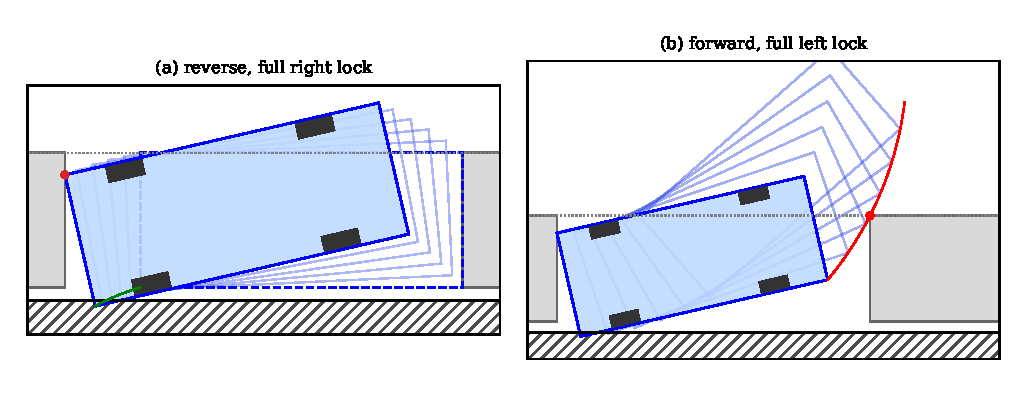
\includegraphics[width=\textwidth]{figures/fig_two_soft.pdf}
\caption{The two-manoeuvre exit of \cref{prop:two-soft} for the typical car ($L=\Lambda_2^{\rm s}=5.312$ m), with tyres drawn.
(a) Reverse with full right lock from the level position touching the car in front (dashed) until the rear bumper touches the car behind; the rear overhang passes over the curb.
(b) Forward exit with full left lock; the front curb-side corner (red trace) grazes $\Qf$.}
\label{fig:two-soft}
\end{figure}

\subsection{Three or more manoeuvres}
For more manoeuvres we repeated the zigzag searches of \cref{sec:zigzag,app:twenty} with the soft-curb collision test (\cref{app:numerics}).
For the typical car they give $\Lmins(3)\le5.088$, $\Lmins(4)\le4.978$, $\Lmins(5)\le4.906$ and $\Lmins(20)\le4.704$ m; \cref{tab:compare} lists all six cars.
The motions differ from the rigid ones.
The reverse manoeuvres are no longer stopped by the rear corner hitting the curb, but by the rear bumper meeting the car behind.
In the five- and twenty-manoeuvre motions of \cref{app:five-soft,app:twenty-soft}, for instance, the car is wedged between the two parked cars rather than between the curb and the car in front (compare \cref{app:five,app:twenty}).
In the twenty-manoeuvre motion the tyres never come closer than $16$ cm to the curb, and the body passes at most $5.2$ cm beyond the curb.

\subsection{Many manoeuvres}

\begin{proposition}\label{prop:asym-soft}
Assume the hypotheses of \cref{thm:asym}, $H<\min(b+\lambda,\,d_b+a)$, $m+\delta_s<w$ and
\begin{equation}\label{eq:mcond-soft}
  w-(m+\delta_s)\sec\psi>\ell\tan\frac\psi2\qquad\text{for }0<\psi\le\psi_{\max}.
\end{equation}
Then \cref{thm:mono,thm:asym} hold for the soft curb, with the same constant $K$.
That is, $\ell<\Lmins(n)\le\Lmins(1)$ for all $n$, and $\sqrt n\,(\Lmins(n)-\ell)\to K$.
\end{proposition}

\begin{proof}
The upper bound $\limsup_{g\to0}g^2N^{\rm s}(g)\le K^2$ follows from \cref{prop:asym-upper} and \eqref{eq:soft-le}.
For the lower bound we go through \cref{sec:asym}.
The curb is used only in \cref{lem:confine}, through lower bounds for the heights of the lowest corners.
In the soft-curb model, $\cTr_y\ge0$ and $\cTf_y\ge0$ give instead
\[
  \cFC_y\ge-\delta_s,\quad \cRL_y\ge(w-\delta_s)\cos\psi-(d_b-\lambda)\sin\psi\qquad(\psi\ge0),
\]
\[
  \cRC_y\ge-\delta_s,\quad \cFL_y\ge(w-\delta_s)\cos\psi-(d_f-\lambda)|\sin\psi|\qquad(\psi\le0).
\]
Hence, in the proof of \cref{lem:confine}(i), $\cRL$ (nose-up) and $\cFL$ (nose-down) still lie above the gap when $|\psi|\le\psi_1$ is small.
In case d and its nose-down analogue, the depth $m-\cFC_y$, respectively $m-\cRC_y$, is now at most $m+\delta_s$ instead of $m$.
The proof goes through with $m$ replaced by $m+\delta_s$ in the constants $c$ and $\psi_1$ and in the function $f$ of part (ii).
Part (ii) uses \cref{lem:soft-fit} instead of \cref{lem:fit}, and \eqref{eq:mcond-soft} instead of \eqref{eq:mcond}.
The rest of \cref{sec:asym} concerns configurations with $u\ge0$ and $|\psi|<cg$.
Their lowest points are at height at least $m-O(g)>0$, so the curb plays no role there in either model.
\end{proof}

Condition \eqref{eq:mcond-soft} holds by a wide margin for all six cars of \cref{tab:cars}.
The two models therefore have the same leading-order asymptotics.

\subsection{The flush problem}
In the soft-curb model the margin may be zero.
The flush problem is then not degenerate, unlike in the rigid model (\cref{prop:flush}).
For $m=0$ and the typical car, a parked car can tilt by at most $\psi_t=0.0073$ rad, which is less than $\beta_t$.
The binding constraint is therefore the swing of the rear tyre during the exit, as for the rear corner in \cref{thm:one}.
Numerically, the best one-manoeuvre exit then needs $5.856$ m.
This is the value $X(\psi)+\sqrt{\rho^2-(r_t-H)^2}$ at the heading $\psi$ with $Y(\psi)=r_t-H$, slightly below the classical $5.861$ m.
The two-manoeuvre exit of \cref{prop:two-soft} is not available for $m=0$, because \ref{T:tyre} fails.
